\documentclass[12pt,letterpaper]{exam}
%\usepackage{color}
\usepackage[usenames,dvipsnames,svgnames,table]{xcolor}
\usepackage[margin=0.9in]{geometry}
\renewcommand{\familydefault}{\sfdefault}
\usepackage{multicol}
\pagestyle{head}
\definecolor{c01}{HTML}{FFBBDD}
\definecolor{c02}{HTML}{FFBBBB}
\definecolor{c03}{HTML}{FFDDDD}
\header{AM 21a Problem Set 01}{Updated on \today.}{Due Thurs Feb 4th @6pm ET}
\runningheadrule
\headrule
\usepackage{diagbox}
\usepackage{graphicx} % more modern
%\usepackage{subfigure} 
\usepackage{amsmath} 
\usepackage{amssymb} 
%\usepackage{gensymb} 
%\usepackage{natbib}
\usepackage{hyperref}
%\usepackage{enumitem}
%\setlength{\parindent}{0pt}
%\usepackage{setspace}
%\pagestyle{empty}  
%\newcommand{\Sc}[0]{
%{\color{BlueViolet}\S}
%}
\usepackage{tcolorbox}
\usepackage[framed,numbered,autolinebreaks,useliterate]{mcode}

\begin{document}
 \pdfpageheight 11in 
  \pdfpagewidth 8.5in

\begin{itemize}
\itemsep0em
    \item Review sections \S 12.1-\S 12.5 in Hughes-Hallett, the course text.
    \item The odd numbered problems in the Exercise sections (the first chunk of problems) in each section are worthwhile practice for before a problem set.  \emph{Answers are in the back for odd numbered problems, and solutions are in the student solutions manual.}
    \item The problems and strengthen your understanding questions are a source of worthwhile practice questions as preparation for quizzes.
\end{itemize}





\begin{questions}
% \item Start using Piazza.  Head to Canvas and choose the Piazza tab.  \begin{itemize}
% \item Post a question or a short note.  You can ask the course staff and fellow students something like ``what was an interesting topic in a previous math course?'' or ``what are you looking forward to in 21a?''.  Label your post with a relevant `tag' (pset01, for example).  Then click around and explore Piazza.  You may want to try writing some mathematics in Piazza using Latex.  Latex allows you to type out mathematics more easily.  Try 
% \begin{verbatim}
% $$ \int f(x)dx $$
% \end{verbatim} 
% for example, or 
% \begin{verbatim}
% $$\frac{df}{dx}$$
% \end{verbatim}
% or look up how to latex a different math expression.

% You are welcome to post anonymously to your fellow students.
% \end{itemize}

\item[0.] In addition to attending office hours, questions about the problem set can be posted to the \#questions channel of the course Slack.  
\begin{itemize}
    \item Submit your problem set work via Gradescope.  Include screenshots of your Matlab work where it is part of the answer to the question.  Work submitted on Gradescope is what will be graded.
    \item When prompted by Gradescope, tag problem parts within your Gradescope submission.
    \item For completeness / academic integrity purposes, submit your matlab source code via Canvas.
\end{itemize}

\item Complete the problems assigned via WeBWorK.  \url{https://courses1.webwork.maa.org/webwork2/harvard-apmth-22b/}

Your username is the text before the @ in your @college.harvard.edu email address.  Your initial password is your HUID.

% interpreting the meaning of a function output.
% distances from points to planes
% equation of largest sphere in first octant
% dimension of space associated with graph, image, level sets
% match functions and graphs in 3-space
% provide names for level surfaces
% match graphs to contour plots
% windmill question
% match level surfaces to functions
% can the level surface be written as the graph of a function of two variables?


\item (Three plot commands) Matlab: I am assuming that you have Matlab installed on your machine, or that you have set up Matlab in the cloud (Harvard has a subscription: \url{https://matlab.mathworks.com}).  If the command \texttt{syms x} does not work, add the symbolic math toolbox to your installation, or switch to \url{https://matlab.mathworks.com}.

\begin{tcolorbox}
\noindent\textbf{Some symbolic toolbox plotting commands}

\texttt{fplot}: plot the graph of a function of one variable, $f(x)$.

\texttt{fplot3}: plot a curve in three-space, $\left(f(t),g(t),h(t)\right)$.

\texttt{fsurf}: plot a surface in three-space, $\left(f(s,t),g(s,t),h(s,t)\right)$.

\texttt{fimplicit}: plot the graph of solutions to an equation $f(x,y) = 0$ (a plot in $2$-space).

\texttt{fimplicit3}: plot the graph of solutions to an equation $f(x,y,z) = 0$ (a plot in $3$-space).
\end{tcolorbox}

You'll use three different plotting methods to make the same plot: \texttt{fsurf}, \texttt{fimplicit3}, and \texttt{surf} (non-symbolic).
\begin{parts}
\item Modify the matlab file, following the instructions below.

\begin{enumerate}
\item Open the matlab file associated with this problem set in the matlab editor (or in an editor of your choosing, but remember to turn on syntax highlighting).
\item Find the \texttt{Section} associated with \texttt{PSet 01, Q01} and run the section.
\item At the command line, use \texttt{doc meshgrid} to look up the meshgrid command.  In line 12, add a comment describing the contents of \texttt{x1} and \texttt{y1}.
\item Right now the plots are in a $n\times 1$ grid.  Edit the code so that they are in a $1\times n$ grid.
\item In the command for the third plot, try \texttt{'='} instead of \texttt{'=='}.  What does \texttt{matlab} tell you about the difference between \texttt{'='} and \texttt{'=='}?  Add a comment about this in line 27, in your own words.
\item Lines 32-42 are formatting the plots.  Comment out the \texttt{axis} command.  Do all of the commands use the same default axes ranges?  Edit the comment in line 35 with your answer.
\item Adjust the axes so that they are tighter on the surface.
\item At the command line, use \texttt{doc caxis}.  What is this command doing?  Edit the comment in line 40 with your answer.
\item Choose a new color range that is too small (so some $z$-values are outside of the range on each side).
\item The \texttt{EdgeColor} of the plots is currently set to green.  Change it to \texttt{'none'}.
\item At the command line, if you type \texttt{plotlist(1).plot.} and then press tab, you'll see a list of plot properties that you can edit \emph{(Note the . after the word plot...}.  Choose \texttt{'FaceAlpha'}, which sets the transparency of the surface.  Make the surface at least $50$\% transparent (choose a number below $0.5$.
\end{enumerate}
\item Print the figure to a file.

On line 44 there is a print command that has been commented out.  Replace my initials with yours, and copy the command part of the line to the command line to export your figure to an eps-file.  \emph{If you are using a Mac the path should work as written.  If you are using a PC, edit the directory listings to match PC syntax.}

\item Print a new figure to a second file.

Change the function from $x^2+y^2$ to a different quadratic function (of your choice).  Run the section (after your edits above) with the new function, and print your new figure (substitute \texttt{p2} for \texttt{p1} in the file name).


\end{parts}

% For reference:

% Hughes-Hallett 12.2 3, 23.  12.3 17, 18, 27, 36.  12.4 12.  12.5 1, 6, 23.  13.1 25, 39

% Stewart 12.6 21

\item (wave travel) A wave travels in an irrigation channel, with $x$ its distance along the channel and $t$ the time.  Let $z$ be the height of the water above a baseline level.  The graph of $z$ as a function of $x$ and $t$ is given below.  

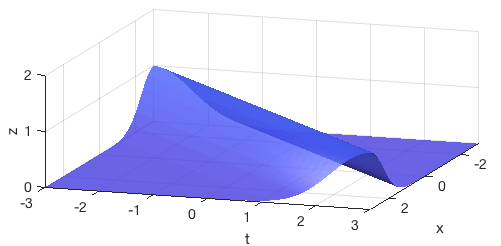
\includegraphics[width=0.5\linewidth]{img/pset02.png}
\begin{parts}
\item Is the plot given in $txz$-space or in $xtz$-space?  \emph{You may want to redraw the positive parts of the axes for yourself.  Then think about the axes labels in analogy to $xyz$-space.  Is $txz$ a right-handed coordinate system or is $xtz$?}.
\begin{solution}
There are a few ways I can think of this: 
\begin{itemize}
    \item If I look down the positive $z$-axis then the plan looks like the $xt$-plane, rather than the $tx$-plane, so it is $xtz$-space.
    \item If my index finger points along the positive $x$-axis and my middle finger points along the positive $t$-axis then my thumb is pointing upward along the positive $z$-axis so $xtz$ is the order tha follows the right hand rule.
    \item It looks like $t$ has been swapped for $y$ in its role, so $xyz$-space becomes $xtz$ space.
\end{itemize}
\end{solution}
\item  Consider the following four functions: $f(x,t) = -(x+t)^2+2$, $f(x,t) = -(x-t)^2+2$, $f(x,t) = e^{-(x-t)^2}$,$f(x,t) = e^{-(x+t)^2}$.  
\begin{itemize}
    \item Find the \texttt{Section} associated with \texttt{PSet 01, Q02b}.  In that section, create code to use \texttt{plot} or \texttt{fplot} to plot two cross-sections for each function, one at $t = 0$ and one at $t=1$.  Make these plots in $xz$-space.
    
    \emph{The command \texttt{hold on} will allow you to add a second plot to the same axes.}
    \item Export your set of plots to \texttt{PSet01Q02p1-yourinitials.eps}.
\end{itemize}
%\item Draw profiles of the wave using $xz$-axes for times $t = 0, 1, 2$ (these are cross-sections).  
% \begin{solution}

% \includegraphics[width=\linewidth]{img/pset02cross.jpg}
% \end{solution}
\item Which of these cross-sections best match the wave above?  Identify the details that you used to make the match.

\item Is the wave traveling in the direction of increasing $x$ or decreasing $x$?  Explain how you decided.

\item Based on the function options I provided, the surface is either a parabolic cylinder or a Gaussian cylinder.  Which is it?


% \begin{solution}
% The peak of the wave is moving in the positive $x$-direction as $t$ increases, so the wave is travelling in the direction of increasing $x$.
% \end{solution}
% \item Which of the following functions is the best match for this plot?

% $f(x,t) = -(x+t)^2+2$, $f(x,t) = -(x-t)^2+2$, $f(x,t) = e^{-(x-t)^2}$,$f(x,t) = e^{-(x+t)^2}$

% Justify your choice using reasoning about cross-sections.
% \begin{solution}
% The first two equations have negative output at some values of $(x,t)$ where our graph shows positive heights.  They correspond to parabolic cylinders.  The next two equations are for Gaussian cylinders.  The center of the peak $e^{-(x-t)^2}$ occurs when $x-t = 0$ so when $x = t$.  The center of the peak $e^{-(x+t)^2}$ occurs when $x+t = 0$ so when $x = -t$.  The option $f(x,y) = e^{-(x-t)^2}$ is consistent with a wave traveling in the positive $x$ direction as $t$ increases, so is the best match.
% \end{solution}
\item Use Matlab to make a plot where the wave is moving in the opposite direction as time increases.

% \begin{solution}
% To reverse the direction of the peak I want to use the function $f(x,y) = e^{(x+t)^2}.$
% Here's the code to plot this:

% \includegraphics[width=\linewidth]{img/pset2cod2.png}

% \includegraphics[width=\linewidth]{img/pset02plot.png}
% \end{solution}
\end{parts}




\question (windmill power)
% This has been moved to Webwork...

The power, $P$ (units of ML$^2$T$^{-3}$), produced by a windmill is proportional to the density of the air pushing the blades, $d$ (units ML$^{-3}$) to the square of the diameter of the windmill, $r$ (units L), and to the cube of the wind speed, $v$ (units LT$^{-1}$).  (M = mass, L = length, T = time).  See 
\url{https://canvas.harvard.edu/files/11684882/}
%\url{http://faculty.buffalostate.edu/sabatojs/courses/GES497/F08/dimensional_analysis.pdf} 
for more information.

%\begin{parts}
% \item Write a formula for $P$ as a function of $d$ and $v$.
% \begin{solution}
% We need $P$ to be proportional to $d^2$ and to be proportional $v^3$.  Choose $k$ as our constant of proportionality.  We have \[P = k d^2 v^3\] as a formula for $P$ that satisfies the conditions we are given.
% \end{solution}
% \item A windmill generates $100$ kW of power at a particular wind speed.  If a second windmill were built with twice the diameter of the original, at what fraction of the original wind speed would it produce $100$ kW?
% \begin{solution}
% A windmill with diameter $d_0$ generates power $100$ at a wind speed $v_0$.  So $ 100 = k d_0^2v_0^3$.  A second windmill has twice the diameter of the first, so $d_1 = 2d_0$.  We'd like to find the fraction of the original windspeed at which this new windmill produces power $100$.  So \[100 = k d_0^2v_0^3 = k(2d_0)^2 (\alpha v_0)^3\] where $\alpha$ is the fraction.  Canceling the constants of proportionality and expanding, we have \[d_0^2v_0^3 = 4\alpha^3 d_0^2v_0^3.\]  Canceling $d_0^2v_0^3$ from both sides, we have $4\alpha^3 = 1$ so $\alpha = 4^{-1/3} \approx 0.63$.  This is about $3/5$ the wind speed to generate the same power if we double the diameter of the windmill.  \emph{Pretty good return...}
% \end{solution}
%\item 
Following the instructions in the WeBWorK problem, sketch a contour diagram for $P$.

\emph{It is fine to make the diagram in Matlab - I don't know how to do the contour labeling via Matlab at the moment, so if you figure it out please let us know via Slack.  Or you can use Matlab to help you figure out the contours that you sketch and label by hand.  Note: stay in a physically plausible range for the values of the variables.}
\begin{solution}
Set $P = nk$ where $ n = 1, 2, 3, 4$ to sketch four contours.  These are curves $k d^2v^3 = n k$, so $d^2v^3 = n$.

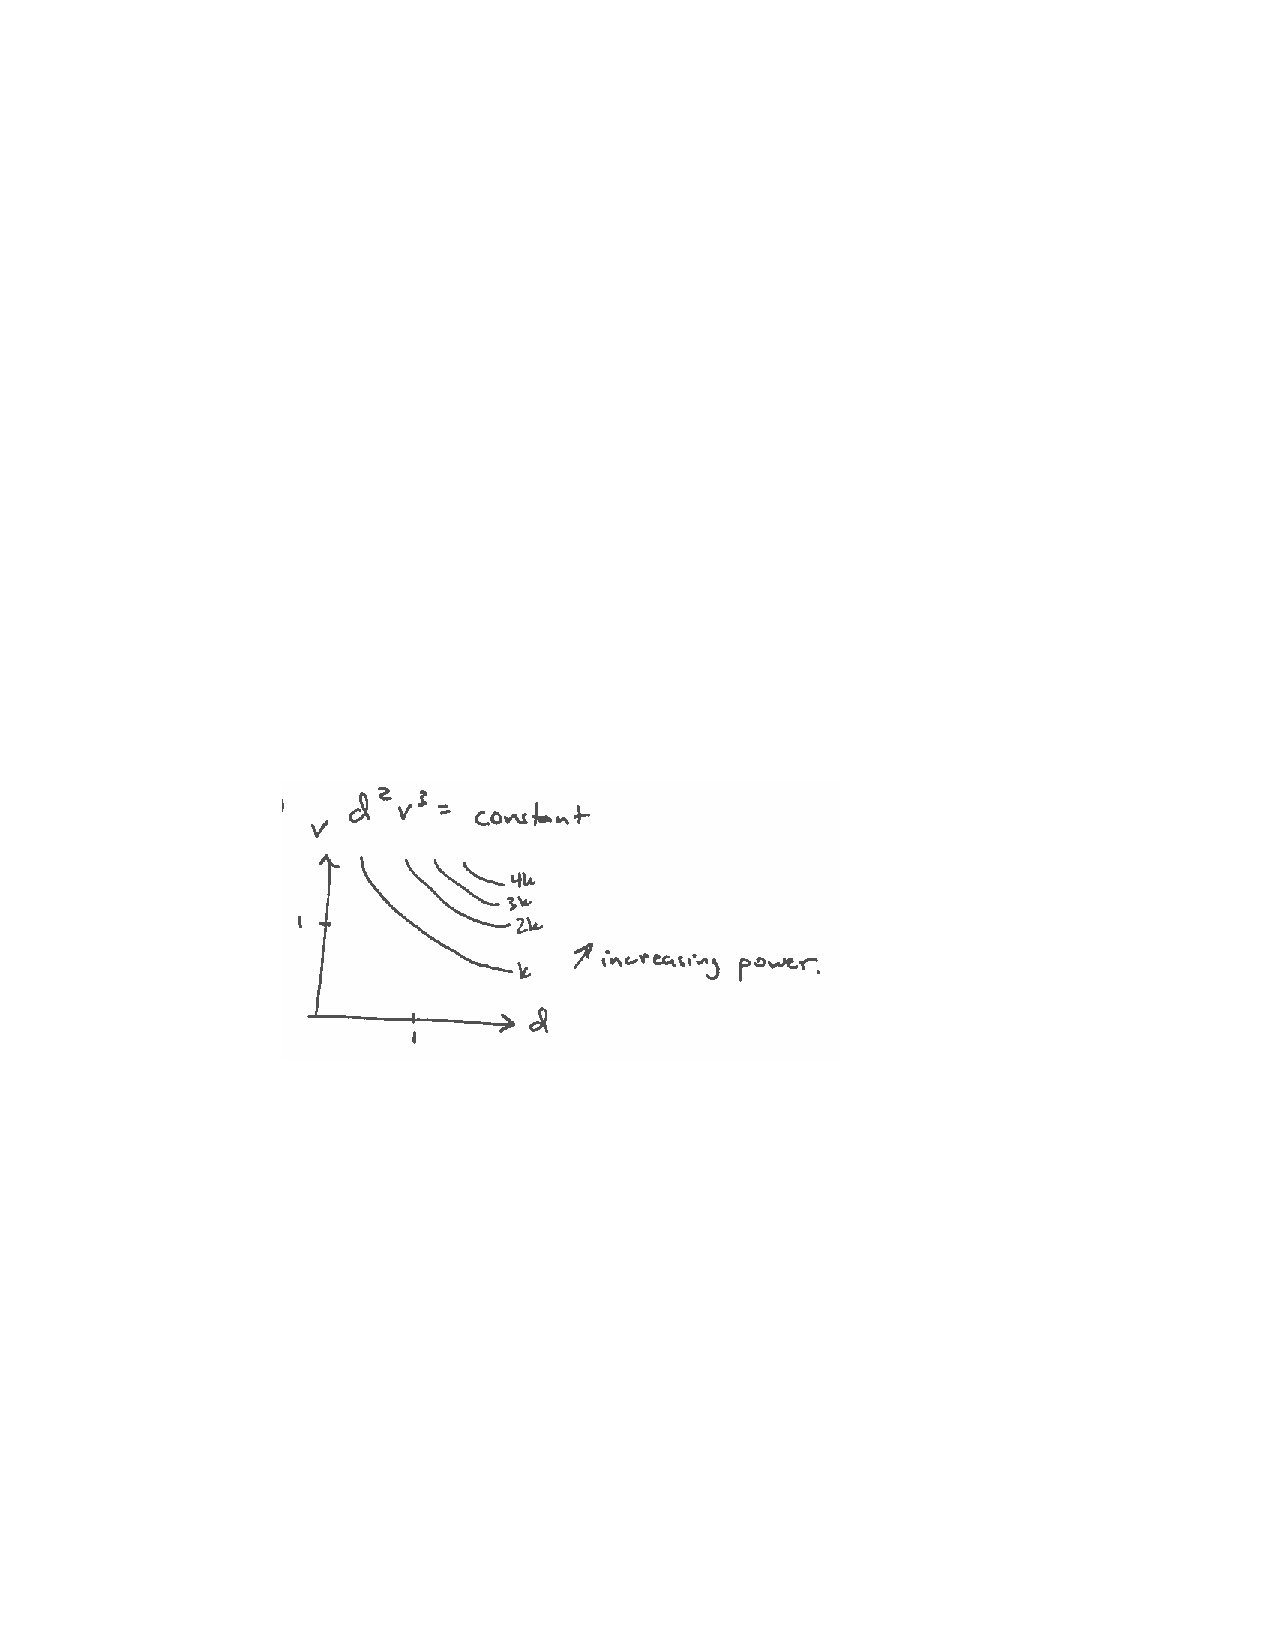
\includegraphics{img/H02contours.pdf}

To find the shape of the curves, I can plug in points: for $n=1$, when $d = 1$ we have $v=1$.  When $d = 1/2$ we have $v = 4^{-1/3}$.  With three points the shape of the first curve comes through.  For the next curves the shape is similar, we just need to know where to put them, so one point is enough.

I can also use the following matlab code to learn the shape of the curves:

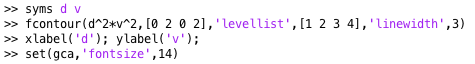
\includegraphics[width=\linewidth]{img/pset02code.png}
\end{solution}
%\end{parts}

\question (coastal Massachusetts contour plot)
You'll try different smoothings to make a contour plot of coastal Massachusetts.  Run lines 57 to 105.  Those will produce an initial contour plot.

\texttt{ALOSMA.tif} holds elevation data (in meters).  Assume that each pixel in the original file represents a region that is 30m by 30m.

\begin{parts}
\item If \texttt{wiener2.m} doesn't run you'll need to install the \texttt{image processing} toolbox.  To do that, head to your Mathworks account, open your individual license file, download the installer, run the installer, and keep proceeding until the installer offers a variety of options.  At that point, choose the image processing toolbox as the one that you'll install.
\item Look up any commands you don't already know using \texttt{doc command-name}.  Make a list of those commands here.
\item Describe, in your own words, what is happening in lines 57 to 105.
\item From line 107 onwards, provide your own code, making your own choices about
\begin{itemize}
    \item downsampling \texttt{imageuse} 
    \item smoothing \texttt{smoothimage}
    \item the contour interval / contour curves to be included in the plot.
\end{itemize}

\end{parts}

\question (land lost to sea level change)
Assuming that sea levels rose by 15 cm over the 20th century (\url{https://www.pnas.org/content/early/2017/05/16/1616007114/tab-figures-data}), approximate how much coastal land in the \texttt{ALOSMA.tif} image was lost to sea level rise during the 20th century.

\emph{You might assume that the slope of the land near the coast is similar on land and under water}.

Describe your assumptions, your approximation method, and your conclusion.  Any associated matlab code should be in the matlab file.

% \item Find a function $f(x,y,z)$ whose level surface $f=3$ is the graph of the function $g(x,y) = x^2 + 2xy$.
% \begin{solution}
% We want the level surface $f=3$ of the function to correspond to the surface given by $z = x^2+2xy$ since this surface is the graph of $g(x,y) = x^2+2xy$.  Rearranging to write the surface as a $3$-level set, we have $z - x^2+2xy + 3 = 3$.  Setting $f(x,y,z) = z-x^2+2xy+3$ gives us a function whose $3$-level surface is the graph of $g(x,y)$, as desired.  Note that there are many other possible functions $f(x,y,z)$ that will work.
% \end{solution}

% \item A drug is injected into a patient's blood vessel.  The function $c = f(x,t)$ represents the concentration of the drug at a distance $x$ mm measured from the point of injection in the direction of blood flow at a time $t$ seconds since the injection.
% \begin{parts}
% \item What are the units of $\frac{\partial c}{\partial x}$ and $\frac{\partial c}{\partial t}$?
% \begin{solution}
% The first has units of concentration per millimeter and the second has units of concentration per second.
% \end{solution}
% % \item Each of these partial derivatives gives an instantaneous rate of change.  Describe in words what each represents.
% \item What do you expect the sign to be of each partial derivative?  Explain your reasoning and answer in complete sentences.
% \begin{solution}
% These really depends on the transport model one chooses for the drug, so the sign you choose and your reasoning need to match, but there is not a unique answer.  I am going to assume that there is a high concentration near the injection site and a lower concentration further away.  This would give us a negative sign to $\frac{\partial c}{\partial x}$ because as I move away from the injection site the concentration is decreasing.

% I am going to assume that there is a high concentration region that is spreading out.  Away from the injection, this leads to a positive sign for $\frac{\partial c}{\partial t}$ because the drug wasn't yet at a particular location or was at a very low concentration, and as the drug spreads, the concentration becomes more even so rises at that downstream point.  Near the injection, the concentration starts high and decreases in time, so this would lead to a negative sign for $\frac{\partial c}{\partial t}$.  Thus with the assumptions I am describing the sign of $\frac{\partial c}{\partial t}$ depends on our location.
% \end{solution}
% \end{parts}

% \item Contours of $f(x,y)$ are shown below, but the values of $f$ on the contour lines have been omitted.  Given that $f_x(P) >0$, find the sign of $f_y(Q)$, explaining your reasoning.

%  \includegraphics{HW03deriv.pdf}
 
%  \begin{solution}
% We know that $f_x(P)>0$, so we know that the function is increasing as we move to the right off of the $f(P)$ contour on which $P$ sits.  This means that the white area between contours to the right of $P$ corresponds to values that are greater than $f(P)$ and the white area to the left of $P$ corresponds to values that are less than $f(P)$.

% At point $Q$, the sign of $f_y(Q)$ is determined by how $f$ would change as we move tiny amounts away from $Q$ in the vertical direction.  Moving up, we move in that white area which corresponds to values less than $f(P)$.  We also need to check what happens when we move down, to make sure that $f_y(Q) \neq 0$.  Moving down from $Q$, we move into the white area corresponding to values greater that $f(Q)$.  This means that $f_y(Q) < 0$ since we increase as we move down and decrease as we move up.
% \end{solution}

\end{questions}


Late work policy:  Because of the unusual circumstances of our semester, all students have access to deadline flexibility when needed.  You may assume that extensions of up to two days will be approved without issue.  Request those via direct message on Slack.  When you request an extension, specify your preferred new deadline for the assignment.

Late WeBWorK is difficult to arrange (it requires a manual override of the course settings), so I suggest planning ahead to complete it on time.

\vspace{1cm} 
\hrule
\vspace{1cm}

\end{document}